\documentclass[11pt,twoside,reqno]{book}

% Language and font stuff
\usepackage[utf8]{inputenc}
\usepackage[english]{babel}
\usepackage{csquotes}
\usepackage[T1]{fontenc}
\usepackage[final]{microtype}
% Formatting
\usepackage[bookmarks]{hyperref}
\usepackage[toc]{appendix}

% Math commands
\usepackage{amsmath,amssymb,amsthm}

\newcommand{\N}{\mathbb{N}}
\newcommand{\R}{\mathbb{R}}
\DeclareMathOperator{\lspan}{span}
\DeclareMathOperator{\tb}{tb}
\DeclareMathOperator{\rot}{r}
\DeclareMathOperator{\cusps}{c}
\DeclareMathOperator{\tpm}{T}
\newcommand{\maxtb}{\overline{\tb}\,}

\newtheorem{mythm}{Theorem}
\renewcommand{\themythm}{\Alph{mythm}}
\newtheorem*{mythmcopy}{Theorem~\ref{thm:mine}}

%\newenvironment{myproof}[1][\proofname]{%
%  \begin{proof}[#1]$ $\par\nobreak\ignorespaces
%}{%
%  \end{proof}
%}

% Bibliography options
\usepackage[backend=biber,
            hyperref,
            doi=false,
            isbn=false,
            sorting=none,
            style=alphabetic]{biblatex}
\renewbibmacro{in:}{}
\addbibresource{sources.bib}

% Figure options
\usepackage{graphicx}
\usepackage[export]{adjustbox}
\def\img{\includegraphics[height=3em, valign=c]}
\def\imgs{\includegraphics[height=2.5em, valign=c]}

% Mathematica listings setup
\usepackage{xcolor}
\definecolor{tenderblue}{HTML}{4477AD}
\definecolor{tenderyellow}{HTML}{99973D}

\usepackage{listings}
\lstdefinestyle{better}{
    identifierstyle=\color{tenderblue},
    keywordstyle=\color{tenderyellow},
    basicstyle=\ttfamily\small,
    breakatwhitespace=false,         
    breaklines=true,                 
    keepspaces=true,                 
    numbersep=5pt                  
}
% Bring on the Behemoth
\usepackage{bardtex}
\styleoption{seniorproject}

\begin{document}

\titlepg{Lagrangian Cobordisms of Legendrian Pretzel Knots with Maximal Thurston-Bennequin Number}{Raphael Walker}{May}{2021}

\abstr


In the study of Legendrian knots, which are constrained by a differential geometric condition, an area of active interest is conditions for the existence of Lagrangian Cobordisms, which are Lagrangian submanifolds stretching between two embedded Legendrian knots.
Some such cobordisms can be constructed by a sequence of basic moves; they are called constructible.
For any topological ribbon knot $T$, one can construct such a cobordism from some Legendran unknot $U$ to a Legendrian representative $K$ of $T$.
We demonstrate a family of ribbon knots for which there exist constructible cobordisms from a stabilized unknot $U$ to a maximal-TB Legendrian representative of the ribbon knot.

\dedic

Dedicated to...

\acknowl

My advisor, Caitlin Leverson...

Howie Qu

\tableofcontents

\startmain

\chapter{Introduction}\label{ch:intro}

% Applications of knot theory
% DNA, 
Mathematical knots are conceptually similar to real twists of thread. But physical knots are of interest because of the friction between strands, while mathematical knots have no such interaction.
Thus the primary question of interest in mathematical knot theory is the identification, classification, and equivalence of knots. By studying the ``universe'' of knots, we study the topology of a 3-dimensional manifold, most commonly Euclidian 3-space $\R^3$. 
Knot theory also has a number of real-world applications in biology and physics, such as in the knotting of DNA, in the folding of proteins, and in fluid dynamics.

We normally define two knots as equivalent if they are smoothly isotopic.
But this is not the only possible equivalence relation, or even the only interesting one. Another that we will make use of in this paper is the existence of a cobordism --- a smooth 2-manifold having two knots as its boundary.
The existence of a cobordism is a much weaker condition than knot equivalence, so it divides the universe of knots into classes (\cite{fox-milnor}).

% Applications of contact geometry
% Maybe mention briefly that contact geometry has applications in phycs, including optics and mechanics
We can also use knot theory to study spaces with more structure than the normal $\R^3$. 
In particular, by the association of a certain plane field (see Definition~\ref{defn:xi}) with $\R^3$, we are able to study \emph{contact manifolds}. Contact geometry is a rich and actively-studied field, with broad applications to physics, including geometric optics and classical mechanics. The knots of interest living in contact manifolds are \emph{Legendrian knots}, whose tangent vectors lie on the plane field.
This gives rise to the equivalence relation of Legendrian equivalence, which is \emph{strictly finer} than that of smooth equivalence.
% The number of peaks is not known.
The structure of these equivalence classes is nontrivial but somewhat understood: from a number of ``maximal'' representatives (in terms of the Thurston-Bennequin number $\tb$ defined in Subsection~\ref{subsec:invariants}, the value of which over all Legendrian representatives is bounded above for any topological knot type), the rest may be obtained by adding additional local twists.

% It is a result of Fuchs and Tabachnikov (\cite{fuchs-tabachnikov}) that if $K$ and $K'$ are smoothly isotopic Legendrian knots, then with sufficient stabilizations they will also be Legendrian isotopic.
% That is, stabilizations.

Moreover, each contact manifold has a canonically associated 4-manifold, equipped with a similar differential condition. Analogous to Legendrian curves in contact 3-manifolds are Lagrangian surfaces in symplectic 4-manifolds, which allow us to define a similar notion of cobordism for Legendrian knots.
This relation is in a sense finer than that of smooth cobordism, as the existence of a Lagrangian cobordism implies the existence of a smooth one, but it is not an equivalence relation on the set of Legendrian knots as it is not symmetric (\cite{chantraine2015}).

Smooth cobordisms have been extensively studied, but much less is known about their Lagrangian counterparts. There are several known necessary conditions for the existence of cobordisms, several of which we will mention here.
First, the existence of a Lagrangian cobordism from $K$ to $\emptyset$ is mutually exclusive with the existence of a Lagrangian cobordism from $\emptyset$ to $K$ (\cite{gromov}).
The existence of a Lagrangian cobordism from $K_-$ to $K_+$ also gives information about many invariants of $K_-$ and $K_+$ (\cite{pan}, \cite{cdrg}, \cite{baldwin}). 
A particularly useful result gives a simple condition on the values of the classical invariants (Subsection~\ref{subsec:invariants}) of $K_-$ and $K_+$ (\cite{chantraine2010}).
In addition to these obstructions, there are diagrammatically-defined sufficient conditions (\cite{bourgeois15}, \cite{lin}, \cite{guadagni}), though it is nontrivial to use these conditions to make general positive statements about the existence of cobordisms.

% State this as a theorem!
The main result of this thesis is an infinite family of knots, $\{P_n\}$, each of which has a maximal-$tb$ Legendrian representative $K$ admitting a Lagrangian cobordism from a suitably stabilized Legendrian unknot $U$. In fact, this allows us to construct cobordisms from $U$ to any stabilization of $K$. In some cases, such as $P_1$, all Legendrian representatives are stabilizations of the maximal representative.
We state the theorem here; the proof of this is the focus of Chapter~\ref{ch:pretzel}.

\begin{mythmcopy}
     Let $P_n = P(3, -3, n)$, for $n$ an integer, and define $\maxtb P_n$ to be the maximal value of the Thurston-Bennequin number over all Legendrian representatives of $P_n$. Then there exists a Legendrian representative $K$ of $P_n$, and a Legendrian unknot $U$ with $\tb K = \tb U = \maxtb P_n$, such that there is a decomposable Lagrangian concordance from $U$ to $K$.
\end{mythmcopy}


This thesis is organized as follows.
In Chapter~\ref{ch:background}, we provide background material on the theory of Legendrian knots: in Section~\ref{sec:knots}, introducing knots in the smooth context; in Section~\ref{sec:legendrian}, laying out the basics of Legendrian knots, their representation, and useful invariants; and in Section~\ref{sec:cobordisms}, defining smooth and Lagrangian cobordisms and briefly summarizing known results on Lagrangian cobordisms.
In Chapter~\ref{ch:pretzel}, we motivate and prove Theorem~\ref{thm:mine}.
In Chapter~\ref{ch:future}, we discuss other classes of knots which are promising candidates for results similar to Theorem~\ref{thm:mine} (i.e., whose maximal-$\tb$ representatives might admit Lagrangian cobordisms from the unknot).
Finally, in Appendix~\ref{ch:appendix}, we provide and explain the Mathematica code that we used to determine $\maxtb$ for the $P(3, -3, n$) family.



\chapter{Background}
\section{Legendrian Knots}

We are interested in defining a certain class of knots called Legendrian Knots. Before we proceed let us give a definition for knots in general, and touch on how we represent them.

\begin{definition}
    A \textbf{knot} is a (smoothly) embedded $S^1$ in $\R^3$. Two knots are said to be \textbf{equivalent} if there exists a (smooth) isotopy of $\R^3$ taking one knot to the other.
\end{definition}
We require that knots be smooth for two reasons. The first is because non-smooth knots can be wild (pathological).
But requiring knots to be finite polygonal chains also excludes the possibility of pathological behavior, so the second reason for knots to be smooth is because further on we will define Legendrian knots using differential geometry, so our knots must be differentiable. 

We generally represent knots by \emph{diagrams}, which are projections of the knot onto a plane, marked at each double point to indicate which strand passes over the other.
Furthermore, diagrams which have no points of intersection of three or more strands, have only a finite number of double points, and in which each strand is locally flat at a double point, are called \emph{regular diagrams}.

\begin{figure}[ht]
    \centering
    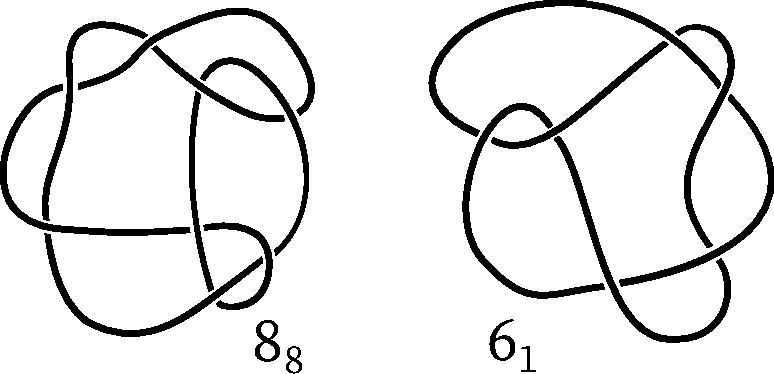
\includegraphics[width=0.45\textwidth]{images/smooth-knots.pdf}
    \caption{Knot diagrams.}%
    \label{fig:diagrams}
\end{figure}

% What is good practice to cite a page number?
Any diagram of a tame (non-wild) knot can be approximated by a regular diagram \cite{murasugi1996}.
Moreover, regular diagrams contain enough information to reconstruct the original knot (up to isotopy). For these reasons it is very convenient to represent knots by regular diagrams, and we will make use of them here frequently.

\subsection{Contact Geometry}

In order to define Legendrian knots we begin by defining a certain plane field on $\R^3$; it is called the \emph{standard contact structure}, or $\xi_0$. At each $(x, y, z) \in \R^3$ we define
\[
    \xi_0(x, y, z) = \lspan \{\partial_y, \partial_x + y\partial_z\}
\]
Note that $\xi_0$ is defined as a linear combination of the partial derivatives of the coordinate functions, as these are the basis vectors of the tangent space $\tpm_{(x, y, z)} \R^3$, of which $\xi_0$ is a 2-dimensional subspace.

\begin{figure}[ht]
    \centering
    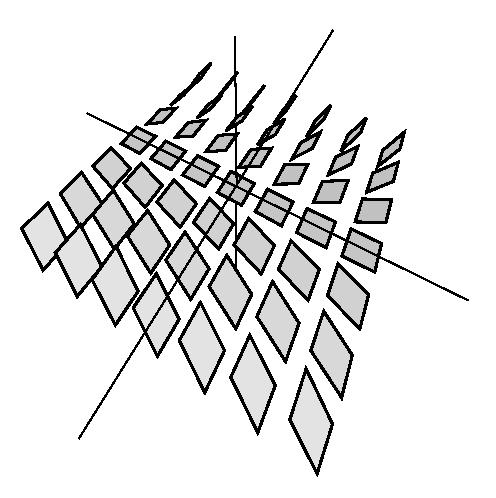
\includegraphics[width=0.5\textwidth]{images/contact-planes.pdf}
    \caption{The standard contact planes in $\R^3$. Diagram from S. Schonenberger.}%
    \label{fig:contact-planes}
\end{figure}
% Add diagram from S. Schonenberger

As we go along the $y$-axis, the plane $\xi_0(p)$  gets steeper and steeper in the $\partial x$ direction. In fact, the planes twist so much that there is no 2-dimensional surface everywhere tangent to $\xi_0$, or even tangent to $\xi_0$ in any open set \cite{boothby}.
% Maybe show the proof with the lie bracket...
Such a plane field is called \emph{completely non-integrable}.
In general, a 3-manifold equipped with a completely non-integrable plane field is called a \emph{contact 3-manifold}.

\textbf{Important!} Every plane field is the kernel of a one-form. In the case of the standard contact planes $\xi_0$, this one form is referred to as $\alpha_0$, and it is given by $\alpha_0 = dz - y \, dx$.

Although no surface can be everywhere tangent to $\xi_0$, there are many curves which run tangent to $\xi_0$. Such a curve is called \emph{Legendrian}, leading to the following definition.

\begin{definition}
    Let $K: (0, 1) \to \R^3$ be a smooth curve. We say $K$ is \textbf{Legendrian} if $K$ is everywhere tangent to $\xi_0$. That is, at all $t \in (0, 1)$,
    \[
        K'(t) \in \xi_0(K(t))
    \]
\end{definition}

As a knot is a smooth embedding of the circle in $\R^3$, so a Legendrian knot is a Legendrian embedding of the circle in $(\R^3, \xi_0)$. But the equivalence relation under which one defines a knot is as important as the curve itself, and so we will define an analogous relation for Legendrian knots. Two knots $K, K'$ are said to be equivalent if there exists a smooth isotopy taking $K$ to $K'$. Similarly, two Legendrian knots $L$ and $L'$ are said to be equivalent if there exists an isotopy taking $L$ to $L'$ such that every intermediate knot is Legendrian.
We frequently use the terms \emph{equivalent} and \emph{isotopic} to refer to knots that are either Legendrian equivalent or smooth equivalent. Generally, when referring to Legendrian knots, we mean Legendrian equivalence, but when confusion may arise we will explicitly use the term \emph{smooth equivalent/isotopic}.

\begin{definition}
    Let $K$ and $K'$ be Legendrian knots. We say $K$ and $K'$ are \textbf{Legendrian equivalent} if there exists a smooth function $\phi: [0, 1] \to \R^3$ such that
    $\phi(0) = K$, $\phi(1) = K'$, and for any $t \in [0, 1]$, $\phi(t)$ is a Legendrian knot.
\end{definition}

By definition, all Legendrian knots are smooth knots, and it is clear that there are representatives of smooth knots which aren't Legendrian. Nonetheless, Legendrian knots are plentiful. In fact, any knot can be $C^0$ approximated by a Legendrian knot (a proof of this fact will be given in section 1.3, once we have defined stabilization).
% TODO: put in this proof 
Such an approximation is smooth isotopic to the target curve, and thus there exist Legendrian representatives of any smooth knot type.

\subsection{Front Diagrams}

Representatives of Legendrian knots are no different from normal knots in that they are curves living in $\R^3$, and so it is convenient to represent them by diagrams.

Unlike smooth knots, Legendrian knots contain geometric information, and so we want our diagrams to record that information too. But because the geometric condition that Legendrian knots satisfy is not invariant under rotation, we must be careful to distinguish which plane we are projecting onto to create a diagram.

There are two projections which are used to represent Legendrian knots. The first is the Lagrangian diagram, which is projection onto the $XY$ plane. This projection is useful in defining certain algebraic invariants, but we will not need it here.
Instead, we restrict our examination to the front projection, which is projection onto the $XZ$ plane such that the positive $Y$ direction points \emph{into} the page.

\begin{figure}[ht]
    \centering
    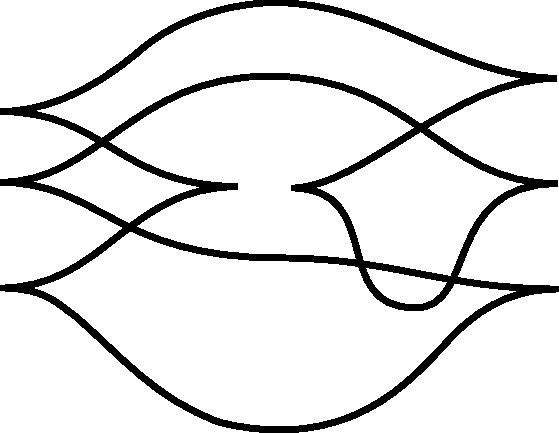
\includegraphics[width=0.3\textwidth]{images/chekanov-1.pdf}
    \hspace{2em}
    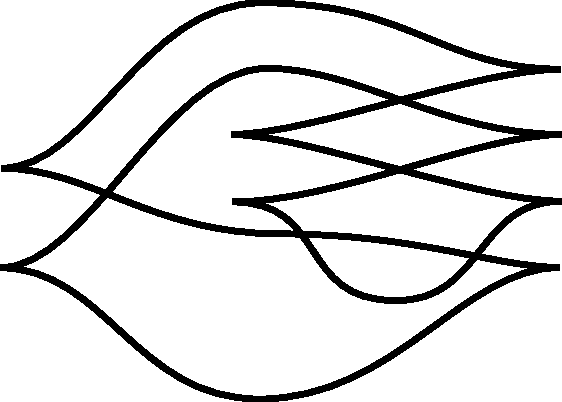
\includegraphics[width=0.3\textwidth]{images/chekanov-2.pdf}
    \caption{Front projections for some Legendrian knots (the Chekanov examples).}%
    \label{fig:front-projection}
\end{figure}

% Could add a proof here..?
Front projections contain enough information to recover the exact geometry of the original knot. This is because the Legendrian condition is a requirement on the tangent based on the $y$-coordinate. Recall that a curve $K$ is Legendrian if $\alpha = dz - y\, dx$ vanishes on $\tpm_p K$ for all $p \in K$. Thus we have $dz - y \, dx = 0$ and thus
\[
    y = \frac{dz}{dx}
\]
This explains the cusps we see on the left and right sides of front diagrams: Since the part above the cusp (which has a negative slope, in the case of a right cusp) and the part below the cusp (which has a positive slope at a right cusp) have to meet, the slopes of each must be zero at the cusp. Note that while these points are cusps in the projection, they are smooth in the 3-dimensional knot.

Moreover, in a front diagram there is no need to mark the overstrand at a crossing: unambiguously, the strand with a more negative slope goes over the other.

\subsection{Classical Invariants}

Any two knots which are Legendrian equivalent are also smooth equivalent by definition, so let us ask whether the converse is true.
As you may expect the answer is no. Moreover, since we can approximate any smooth knot by an isotopic Legendrian one, the relation of Legendrian equivalence ``refines'' the equivalence classes of smooth knots into a larger number of Legendrian equivalence classes. What does the structure of this refinement look like? As expected this is a nontrivial question. We will begin to answer it by looking at equivalence of diagrams.

Although one defines two smooth knots to be equal if there is an isotopy between them as curves in $\R^3$, the Reidemeister moves provide an equivalent \emph{diagrammatic} formulation.
It is three ``moves'' which may be made on a diagram, such that two knots are equal if and only if their diagrams may be related using some series of Reidemeister moves.
The Reidemeister moves don't preserve Legendrian equivalence, but there's a similar set of three diagrammatic moves which determine Legendrian equivalence of front diagrams  \cite{swiatkowski}.

\begin{figure}[ht]
    \centering
    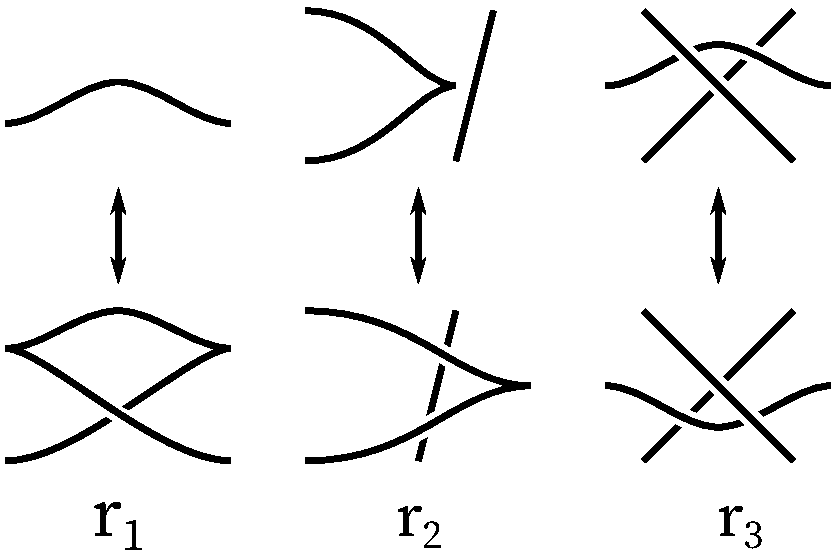
\includegraphics[width=0.5\textwidth]{images/redeimeister.pdf}
    \caption{The Legendrian Reidemeister moves.}%
    \label{fig:redemeister}
\end{figure}

These moves correspond to restricted version of the smooth Reidemeister moves.
Unfortunately, as with the smooth Reidemeister moves, it is difficult in practice to determine equivalence of knots using these rules. Nonetheless, they are useful in the construction of more practical invariants, as invariance under all three Reidemeister moves is equivalent to invariance under Legendrian isotopy.

There are two numerical invariants which can be easily defined in and computed from the front projection, and they are called the \emph{classical invariants}.
\begin{definition}
    Let $K$ be a Legendrian knot, and $D$ a front diagram for $K$. Let $\cusps_r(D)$ be the number of right cusps in $D$, and $w(D)$ the writhe of $D$, defined below.
    Define the \textbf{Thurston-Bennequin number} as
    \[
        \tb(K) = w(D) - \cusps_r(D)
    \]
\end{definition}
To define the writhe $w(D)$ of a diagram $D$, we assign a sign to each crossing in $D$. If as you travel along the overstrand, the understrand goes from right to left, then the crossing is positive; and if the understrand runs from left to right then the crossing is negative. The writhe is the sum of the signs of the crossings.

\begin{figure}[ht]
    \centering
    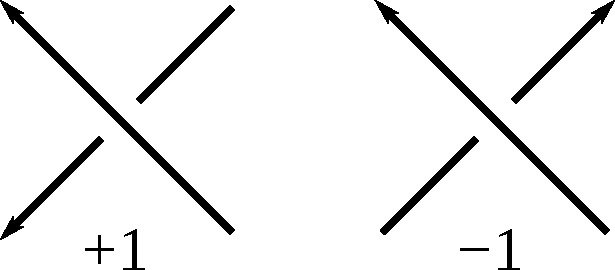
\includegraphics[width=0.3\textwidth]{images/writhe.pdf}
    \caption{The sign at a crossing.}%
    \label{fig:writhe}
\end{figure}

Writhe is \emph{not} an invariant of Legendrian knots. Because the $r_1$ move adds a crossing without changing the orientation of other crossings, it changes the writhe. Nonetheless, the $\tb$ is easily shown to be an invariant.

\begin{proposition}
    The Thurston-Bennequin number is an invariant of Legendrian knots.
\end{proposition}
\begin{proof}
    Let $D$ be a front diagram for a Legendrian knot $K$. It suffices to show that $\tb(D)$ is unchanged under the Legendrian Reidemeister moves.

    \begin{enumerate}
        \item $r_1$ adds one right cusp and one crossing. Regardless of the orientation of of the segment before the move, the new crossing is easily seen to have sign $+1$, and therefore
            \[
                \tb(D') = (w(D) + 1) - (\cusps_r(D) + 1) = \tb(D)
            \]
        \item $r_2$ adds two crossings, but they have opposite signs, so the writhe remains the same.
        \item $r_3$ moves two crossings, but their signs remain unchanged.
    \end{enumerate}
    
\end{proof}

\begin{definition}
    Let $K$ be a Legendrian knot and $D$ a front diagram for $K$. Let $\cusps_u(D)$ be the number of \emph{upward-pointing cusps} and $\cusps_d(D)$ be the number of \emph{downward-pointing cusps}. Define the \textbf{rotation number} of $K$ as 
    \[
        \rot(K) = \frac{1}{2} (\cusps_d(D) - \cusps_u(D))
    \]
    Although $\rot(K)$ is only well-defined for \emph{oriented} $K$, it is defined up to multiplication by $\pm 1$ for unoriented knots.
\end{definition}
\begin{proposition}
    The rotation number is an invariant of Legendrian knots.
\end{proposition}
\begin{proof}
    As before, we show that $\rot(K)$ is an invariant, so let $D$ be a front diagram for $K$. Neither $r_2$ nor $r_3$ change the orientation or the number of cusps. On the other hand, $r_1$ creates a pair of cusps, one pointing upward and one pointing downward.
\end{proof}

These invariants do a good job of distinguishing Legendrian knots (see \cite{eliashberg2008unknot}), though there are known to be pairs of smooth-isotopic Legendrian knots which have the same TB and rotation number but which are not Legendrian equivalent (\ref{fig:front-projection}, \cite{chekanov}). But the existence of these invariants reveals a great deal about how the Legendrian equivalence classes of a smooth knot are structured. 

\begin{figure}[ht]
    \centering
    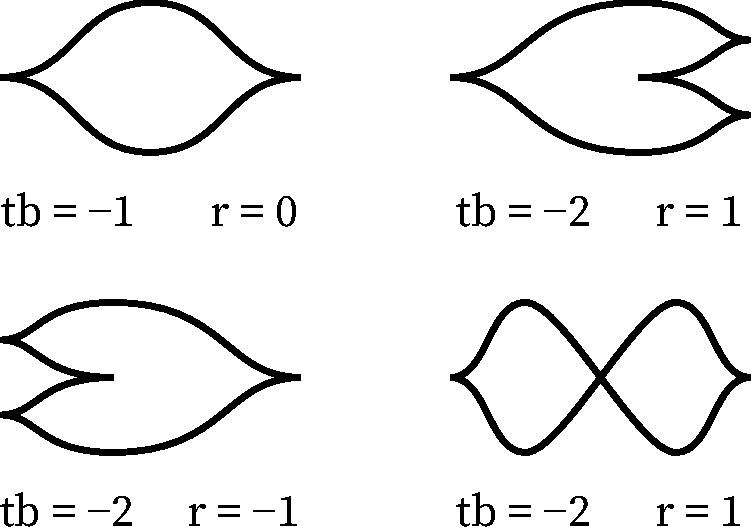
\includegraphics[width=0.4\textwidth]{images/unknots.pdf}
    \caption{A selection of Legendrian unknots.}%
    \label{fig:unknots}
\end{figure}

% Awk
Figure \ref{fig:unknots} shows four Legendrian unknots. One of them has $\tb = -1$ and another has $\tb = -2$, so they aren't isotopic. But the second can be obtained from the first by means of a so-called \emph{stabilization}, shown in figure \ref{fig:stabilization}. 

\begin{figure}[ht]
    \centering
    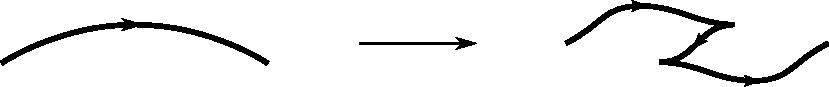
\includegraphics[width=0.6\linewidth]{images/stabilization.pdf}
    \caption{A ``right'' stabilization, increasing the rotation number.}%
    \label{fig:stabilization}
\end{figure}

% Do you need to explicitly mention that stabilization preserves smooth knot type?
A stabilization decreases the TB by 1, and changes the rotation number by $\pm 1$ depending on the orientation. Thus for any topological knot, the TBs of its Legendrian representatives are unbounded below, and the rotation numbers are unbounded both above and below.

It is known that for any topological knot, the TB is bounded above \cite{bennequin}, and therefore the maximal TB is a knot invariant, which we denote $\maxtb(K)$.
For example, the maximal TB for the unknot is $-1$, as seen in Figure \ref{fig:unknots}, and all other representatives are (Legendrian isotopic to) stabilizations of the uncrossed unknot \cite{atlas}. It is possible to determine whether a Legendrian knot is a stabilization using the Chekanov-Eliashberg DGA, but this does not in general determine $\maxtb$: there exists a Legendrian representative of $m(10_{139})$ with $\tb = -17$ and $\rot = 4$ which is not a stabilization of the maximal-tb representative, which has $\tb = -16$ and $\rot = 1$. Thus we have to look elsewhere to determine $\maxtb$.

\subsection{Polynomial Invariants and Skein Relations}

Many useful knot invariants take the form of Laurentian polynomials (ie, having both positive and negative exponents). Typically, these are defined recursively using skein relations, which give an algebraic relationship between the polynomials of knots differing only at a crossing. For certain such relations the resulting knot can be shown to be not only unique, but invariant under isotopy.

In particular, we are interested in the Kauffman polynomial, as it gives an upper bound on the maximal TB of a smooth knot type. We define the Kauffman polynomial in terms of the L-polynomial, which is an invariant only under regular isotopy.
There are many varying definitions of the Kauffman polynomial in the literature. We use here a variant known as the Dubrovnik polynomial (it was discovered in the city of Dubrovnik in Yugoslavia \cite{kauffman}), and we refer to its normalized version as the Kauffman polynomial. Our formulation matches that used by \cite{ferrand} and is similar to that used by \cite{lu-zhong}.

Let $T$ be a knot diagram or an oriented link diagram, and define $D$ recursively via the following skein relations, where $\delta = \frac{a - a^{-1}}{z} + 1$.
\begin{align}
    D\left(\Lmin\right) - D\left(\Lplus\right) &= z \left( D\left(\Lzero\right) - D\left(\Linf\right) \right) \\
    D\left(\Lr\right) &= a D \Big(\Ln\Big)\\
    D\left(\Lu\right) &= \delta
\end{align}

The first two equations are local, indicating a relation between the Dubrovnik polynomials of diagrams which are identical except for the substitution of the indicated figures. The third equation normalizes the recurrence relation by determining the Dubrovnik polynomial of an uncrossed diagram for the unknot. The choice of $\delta$ for the polynomial of the unknot is natural; it arises from setting $D(\emptyset) = 1$ for the empty link.

Yet such a polynomial is certainly not a topological invariant: the $r_1$ move corresponds to multiplication by $a^{\pm 1}$. Thus we normalize the D-polynomial by the writhe to get the Kauffman polynomial $Y(K)$, since the same $r_1$ move which corresponds to a multiplication by $a$ in the Dubrovnik polynomial increases the writhe by 1. This is why we require that $K$ by oriented if it is a link and not a knot: writhe is well-defined for unoriented knots but not for unoriented links in general.
\begin{definition}
    Let $K$ be a knot or an oriented link and $T$ a diagram for $K$. Define the \textbf{Kauffman Polynomial} of $K$ by
    \[
        Y(K) = a^{-w(T)} D(T)
    \]
    The polynomial, which is a Laurentian polynomial in $a, x$, is an invariant under smooth isotopy \cite{kauffman}.
\end{definition}

The degree of the framing variable $a$ in the Kauffman polynomial gives rise to an upper bound on the TB, which was first proved by Rudolph \cite{rudolph}. The version we use here is due to Tabachnikov \cite{tabachnikov}. More information on this bound and its history can be found in \cite{ferrand}.

\begin{theorem}[Kauffman Bound \cite{tabachnikov}]\label{kauffman-bound}
    If $K$ is a Legendrian link, then $\overline{tb}(K) \leq \mu_a(Y(K))$, where $\mu_a(P)$ denotes the minimum degree of $a$ in the polynomial $P(a, x)$.
\end{theorem}

This bound is very useful: there is no method in general for computing the maximal TB of a knot, but it is a fairly straightforward matter to compute its Kauffman polynomial. The bound fails to be sharp in some known cases (eg, \cite{ferrand}) but there are also classes of knots for which it is known to be sharp. These include positive knots, most torus knots, 2-bridge links, and most 3-twist pretzel links. That the Kauffman bound is sharp for many 3-twist pretzel links is a theorem of Ng:

\begin{theorem}[\cite{ng}]
    Suppose $p_1, p_2, p_3 > 0$. Then the Kauffman bound is sharp for the pretzel links $P(p_1, p_2, p_3)$, $P(-p_1, p_2, p_3)$, and $P(-p_1, -p_2, -p_3)$, and for $P(-p_1, -p_2, p_3)$ when $p_1 \geq p_2 \neq p_3 + 1$.
\end{theorem}

We will make use of this theorem in our main result.

\section{Lagrangian Cobordisms}

\subsection{Symplectic Geometry}

Cobordisms are objects originating in smooth knot theory which define a fundamental relation between types of knots. We define them here in the context of smooth knots, and then we will be able to define a type of cobordism called a Lagrangian cobordism by requiring that it be everywhere tangent to a certain differential form.

\begin{definition}
    Let $K$ and $K'$ be smooth knots. Define a \textbf{cobordism} as a smoothly embedded 2-manifold $A$ in $\R^3 \times I$ such that the bottom edge of $A$ is $K$ and the top edge of $A$ is $K'$. That is,
    \begin{align*}
        A \cap \left(\R^3 \times \{0\}\right) &= K \times \{0\}\\
        A \cap \left(\R^3 \times \{1\}\right) &= K' \times \{1\}
    \end{align*}
\end{definition}

We extend this definition by defining a \emph{symplectic manifold} in much the same way we defined a contact manifold: as a manifold equipped with an appropriate differential form. Recall that a 2-form $\omega$ on a manifold $X$ is \emph{closed} if $d \omega = 0$ (ie, its exterior derivative vanishes) and \emph{nondegenerate} if $\omega(\vec v, \vec w) = 0$ for all $\vec w \in \tpm_p X$ implies $\vec v = 0$.

\begin{definition}
    Let $X$ be a 4-dimensional smooth manifold and $\omega$ a two-form on $X$ that is closed and nondegenerate. Then the pair $(X, \omega)$ is said to be a \textbf{symplectic 4-manifold}.
\end{definition}

Analogous to Legendrian curves in contact manifolds are Lagrangian surfaces in symplectic manifolds.
\begin{definition}
    Let $(X, \omega)$ be a symplectic 4-manifold and $L$ a smoothly embedded 2-manifold in $X$. We say $L$ is \textbf{Lagrangian} if for all $p \in L$, $\omega$ vanishes on $\tpm_p L$.
\end{definition}

% This section could do with a rework -- either go more into depth or less into depth.

% give a citation for this
Given a contact manifold $(Y, \ker \alpha)$ there is a canonically associated symplectic manifold $(Y \times \R, d(e^t \alpha))$, where $t$ is the coordinate on the attached copy of $\R$. This allows us to put Legendrian knots into symplectic manifolds as slices of Lagrangian submanifolds. Thus a Lagrangian cobordism is a cobordism that is also Lagrangian, with a few extra conditions required.

\begin{definition}
    Let $K$, and $K'$ be Legendrian links, and $L$ a Lagrangian manifold in $(\R^3 \times \R, d(e^t \alpha))$. We say $L$ is a \textbf{Lagrangian cobordism} between $K$ and $K'$ if for some $T > 0$,
    \begin{align*}
        L \cap \left(\R^3 \times (-\infty, -T)\right) &= K \times (-\infty, -T)\\
        L \cap \left(\R^3 \times (T, \infty)\right) &= K' \times (T, \infty)\\
        L \cap \left(\R^3 \times [-T, T] \right)\, &\,\, \text{is compact}
    \end{align*}
    and there exists a function $f: L \to \R$ such that $df = e^t \alpha |_{\tpm L}$ and $f$ is constant above $t = T$ and below $t = -T$.

    We call a Lagrangian cobordism between two \emph{knots} (excluding links with multiple components) with genus zero a \emph{concordance.}
\end{definition}

\begin{figure}[ht]
    \centering
    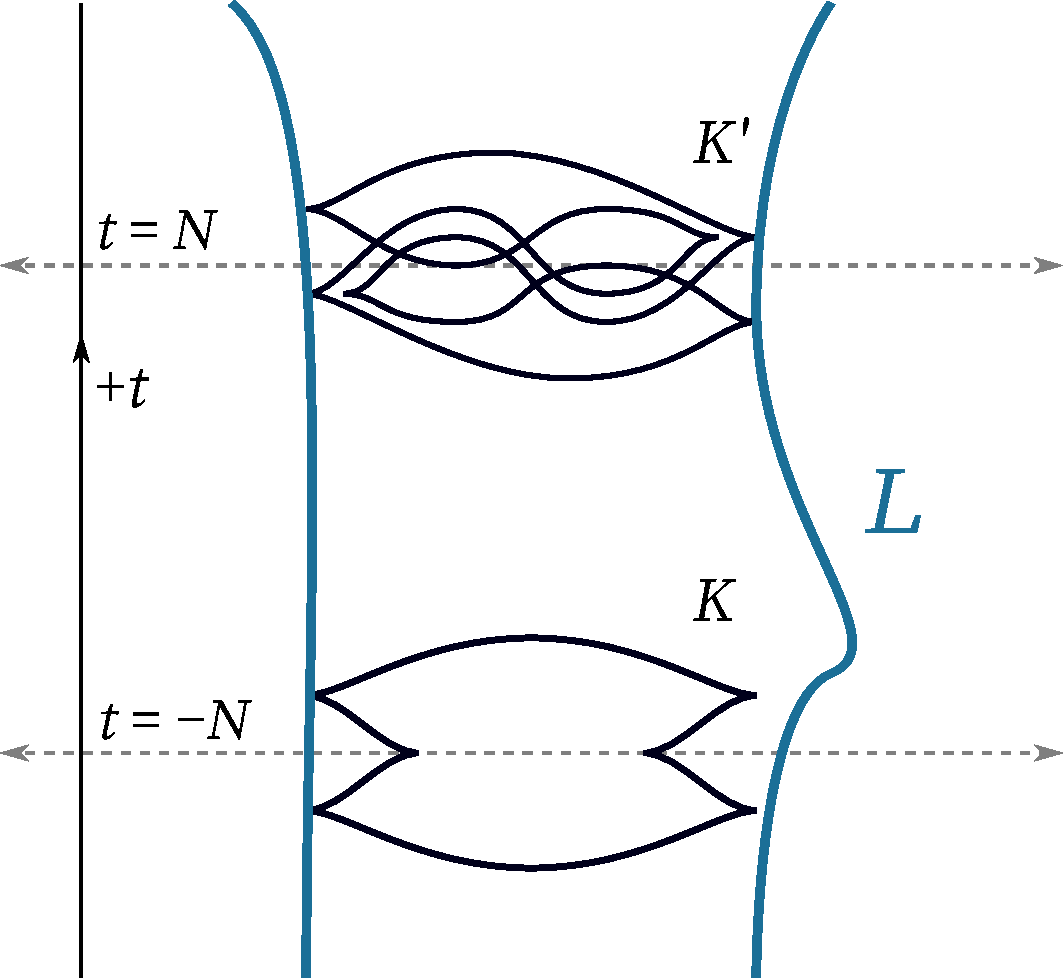
\includegraphics[width=0.4\textwidth]{images/cobordism-visualization.pdf}
    \caption{A visualization of a Lagrangian cobordism $L$ as a cylinder with two Legendrian knots at the ends. Each slice along the $t$ axis is an entire $\R^3$. In this diagram $K$ is the unknot and $K'$ is $m(6_1)$.}%
    \label{fig:cobordism-vis}
\end{figure}

% be more precise here
The change in definition from looking at intersections of the cobordism with $\R^3$-planes to looking at intersections with entire rectangular regions is due to the differential structure of the symplectic manifold; it does not change the nature of the relation. What is more important is that we have added an asymmetric geometric condition on the cobordism, and the result is that the relation "there exists a Lagrangian cobordism from $K$ to $K'$" is not symmetric.

We make the distinction between cobordisms with genus and concordances because the genus of a cobordism gives a lot of information about the two knots at its ends \cite{chantraine2010}. In particular, if $L$ is a cobordism between $K$ and $K'$, then
\[
    \rot(K) = \rot(K') \text{     and     } \tb(K) - \tb(K') = \chi(L)
\]
Thus a Lagrangian concordance can only exist between two knots with equal rotation number and TB.


\subsection{Constructable Cobordisms}

In general, Lagrangian cobordisms are difficult to find. However, there are several conditions in which they are known to exist. Of interest is a certain set of moves which may be easily defined on front diagrams, the Reidemeister moves among them, such that a Langrangian cobordism exists between knots related by them.

\begin{theorem}[\cite{bourgeois15}]
    Suppose $K$ and $K'$ are Legendrian knots. If the front diagram of $K'$ can be obtained from the front diagram of $K$ by a finite sequence of handle moves (figure \ref{fig:handles}) and Reidemeister moves (figure \ref{fig:redemeister}), then there exists a Lagrangian cobordism from $K$ to $K'$. 
\end{theorem}
\begin{figure}[ht!]
    \centering
    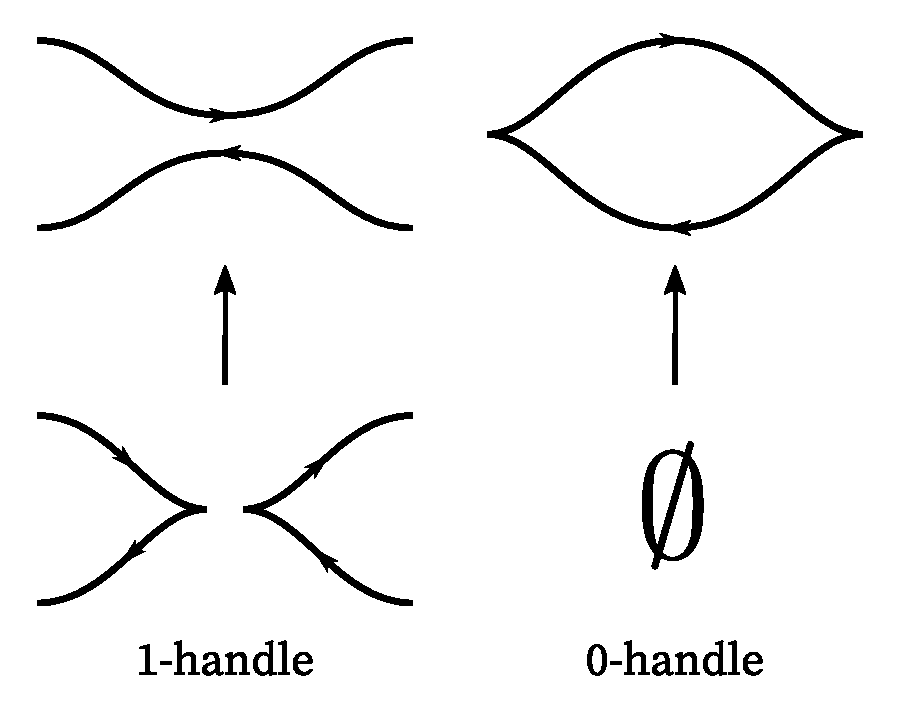
\includegraphics[width=0.4\textwidth]{images/handles.pdf}
    \caption{The handle moves. Note that these moves are one-directional, unlike the Reidemeister moves. The addition of a one-handle is sometimes referred to as a \emph{pinch move}. The addition of a zero-handle corresponds to adding an unlinked unknot with maximal TB to the diagram.}
    \label{fig:handles}
\end{figure}

We refer to a cobordism that is a result of a sequence of these moves as \textbf{constructible}. We can represent these cobordisms visually via a sequence of front diagrams of Legendrian links, each of which is obtained from the previous by one of the constructible moves. For example, figure \ref{fig:cobordism-construction} shows a movie for a constructible cobordism from a double-stabilized unknot to a Legendrian representative of $m(6_1)$.

\begin{figure}[ht!]
    \centering
    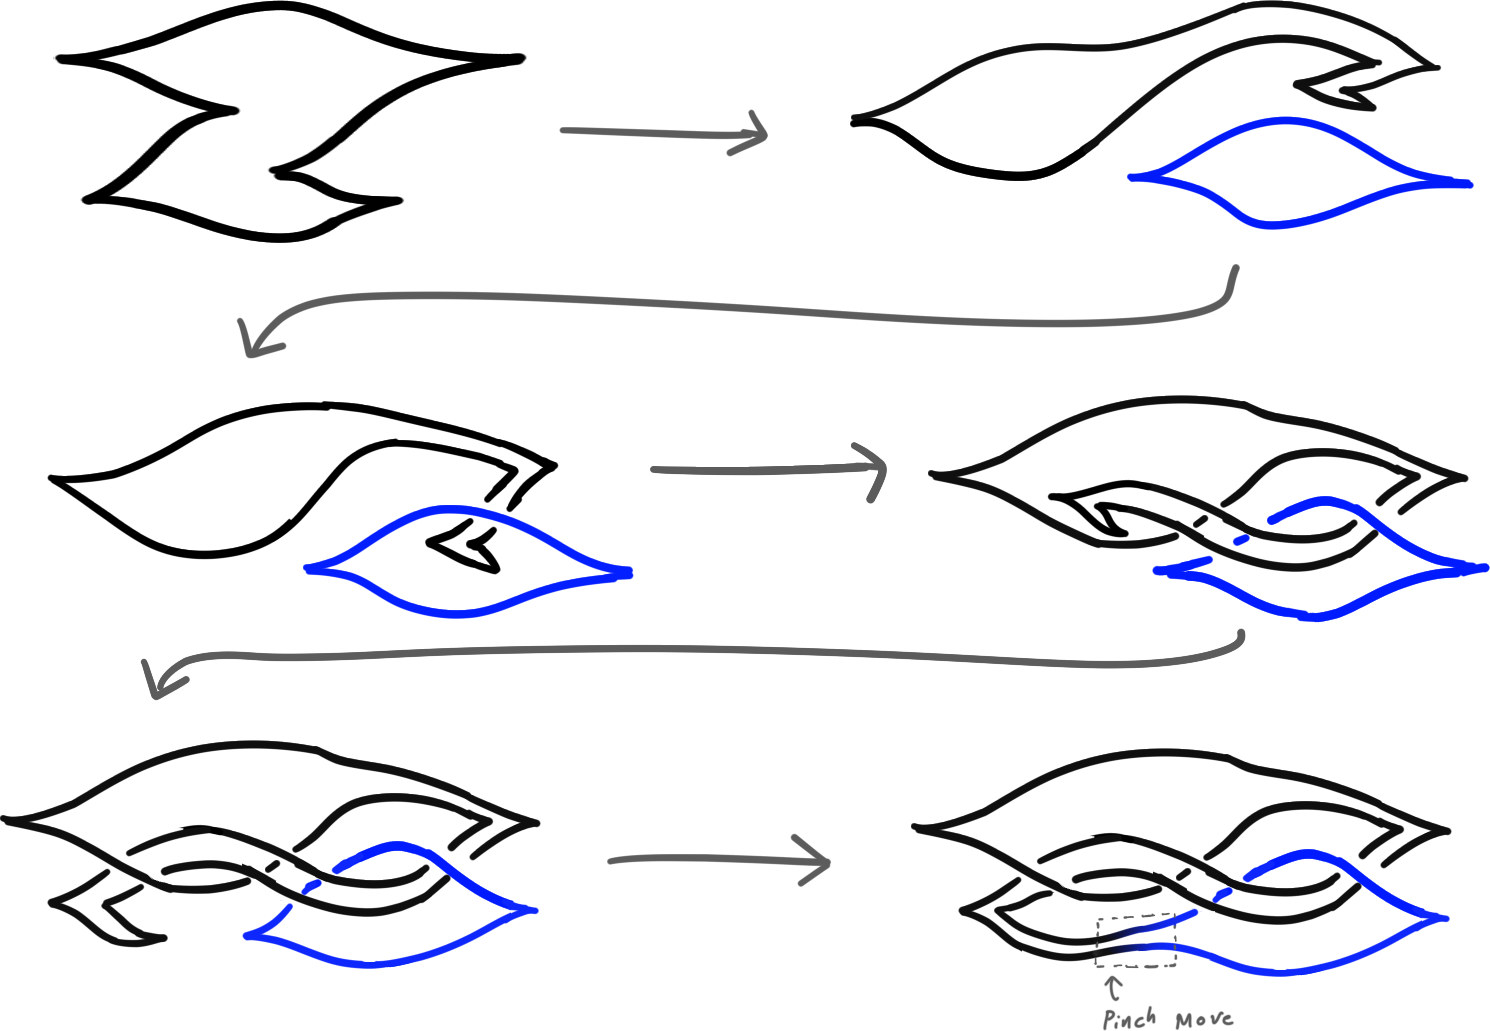
\includegraphics[width=0.5\textwidth]{images/cobordism-construction.png}
    \caption{Constructing a cobordism from the unknot to $m(6_1)$.
    TODO: Make a real nice SVG diagram for this.}%
    \label{fig:cobordism-construction}
\end{figure}

It is known that not all Lagrangian cobordisms are constructible. Moreover, there exist pairs of knots $K, K'$ such that a Lagrangian cobordism exists from $K$ to $K'$ but no such constructible cobordism exists. Specifically, there exists a Lagrangian cobordism from the unknot to the empty set, despite the fact that no constructible move can give $\emptyset$ from a nonempty Legendrian. It is not known whether this is the case when $K' \neq \emptyset$.

\section{Ribbon, Pretzel, etc}

Finding Langrangian cobordisms is hard, and it's not much easier to even know when they exist.
A natural way of refining this question is to restrict one of the knots.
Specifically, we want to know under what conditions there exists a constructible cobordism from the unknot $U$ to some Legendrian knot $K$. TODO: Explain more about this question.

A good candidate for this search is the class of knots called ribbon knots, which we define here.

\begin{definition}
    A knot $K$ is said to be \textbf{ribbon} if $K$ bounds a smoothly embedded disk $d: D \to \R^3$ with only ribbon singularities.
    That is, every region of self-intersection of $d$ is an arc $A \in \R^3$ such that the preimage of $A$, $d^{-1} (A)$, consists of two arks in $D$ of which one is within the interior of $D$ and the other has its endpoints on the boundary of $D$.
\end{definition}

This definition is more clear alongside a ribbon diagram.

\begin{figure}[ht!]
    \centering
    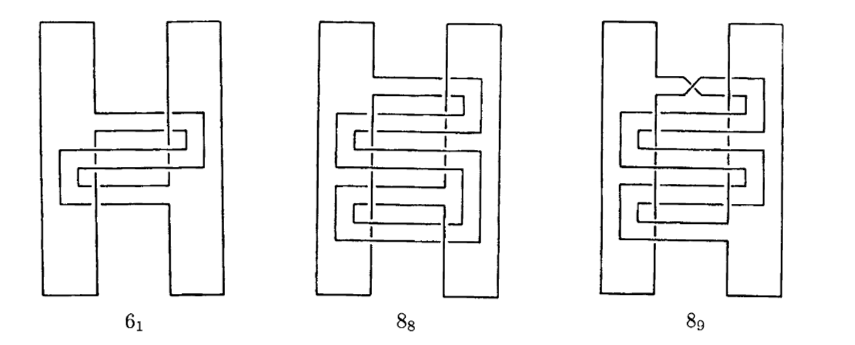
\includegraphics[width=0.8\linewidth]{images/ribbon-knots-kawauchi.png}
    \caption{Ribbon Diagrams, from Kawauchi. TODO: Make your own}%
    \label{fig:ribbon-knots-kawauchi}
\end{figure}

In the smooth world, there are fundamental connections between ribbon knots and cobordisms \cite{fox-milnor}. TODO: Explain this



\chapter{The \texorpdfstring{$P(3, -3, n)$}{P(3, -3, n)} family}\label{ch:pretzel}
\section{Motivation}\label{sec:motivation}
There is no general method of finding Lagrangian cobordisms, and there are very few sufficient conditions for their existence.
A natural way of refining this question is to restrict either $K_-$ or $K_+$.
In particular, we want to know under what conditions there exists a decomposable cobordism from the unknot $U$ to some Legendrian knot $K$. This choice is not arbitrary: it is unclear whether any of the known obstructions give information about the existence of such cobordisms when $\maxtb K \leq -1$.

A good candidate for this search is the class of knots called ribbon knots, which we define here.

\begin{definition}
    A knot $K$ is said to be \textbf{ribbon} if $K$ bounds a smoothly embedded disk $d: D \to \R^3$ with only ribbon singularities.
    That is, every region of self-intersection of $d$ is an arc $A \in \R^3$ such that the preimage of $A$, $d^{-1} (A)$, consists of two arcs in $D$ of which one is within the interior of $D$ and the other has its endpoints on the boundary of $D$.
\end{definition}

This definition is more clear alongside a ribbon diagram, Figure~\ref{fig:ribbons}.

\begin{figure}[ht!]
    \centering
    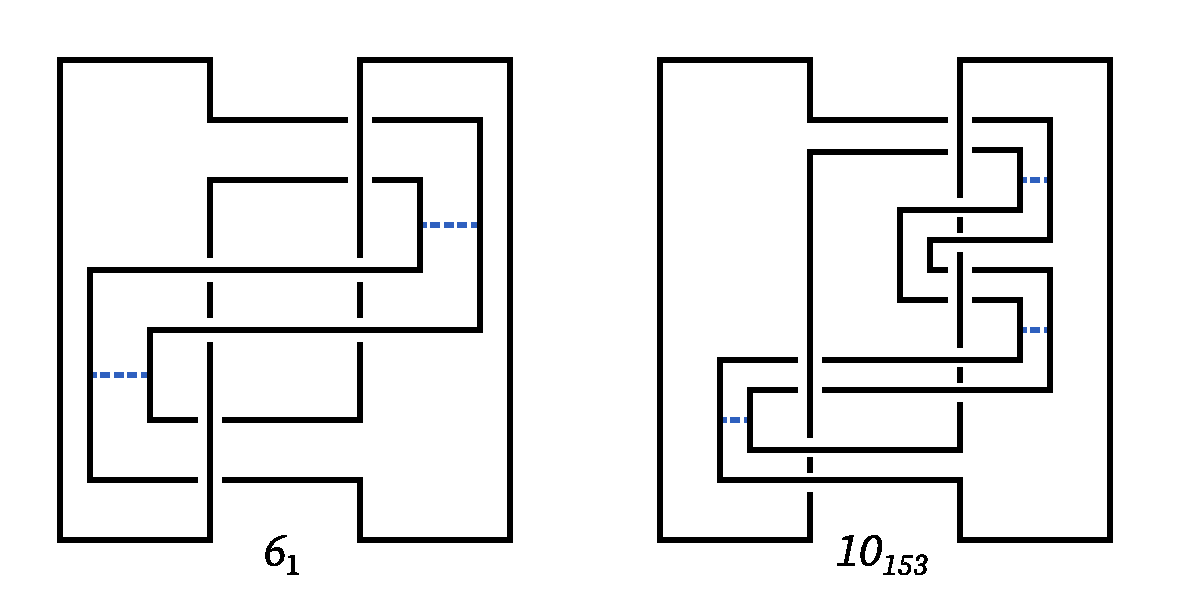
\includegraphics[width=0.6\linewidth]{images/ribbons.pdf}
    \caption{Diagrams for some ribbon knots, with the arcs of self-intersection marked with dashed lines. The forms of these ribbons come from \cite{kawauchi}.}
    \label{fig:ribbons}
\end{figure}

Ribbon knots are a natural class to try to find Lagrangian cobordisms to, as topologically there always exist smooth cobordisms between the unknot and any ribbon knot (recall that the existence of  a Lagrangian cobordism from $K_-$ to $K_+$ implies the existence of a smooth cobordism between the two).
In the case of Legendrian knots, it is known that ribbon knots admit decomposable Lagrangian cobordisms from sufficiently stabilized unknots \cite{leverson-etnyre}.
For a ribbon knot with one band, we can start from a twisted Legendrian unknot, add a second unknot with a 0-handle, and then use Legendrian isotopy to "pass" the tip of the first unknot through the two loops however desired, before finally using a 1-handle to join the ribbon tip to the second unknot, thus closing the knot. 

The cobordism created by these moves is necessarily a concordance: Each 0-handle adds a separate component to the link, and the 1-handle only adds genus if between two points on the same component.
Thus to construct such a cobordism to a Legendrian ribbon knot $K$, we have to start with a Legendrian unknot $U$ with $\tb U = \tb K$. Given the topological knot type of $K$, both $U$ and $K$ must certainly have $\tb \leq \maxtb K$.
It is an open question when this can be achieved with equality: that is, when a cobordism can be constructed from a stabilized unknot to a maximal-$\tb$ Legendrian ribbon knot.

\section{Constructions of Cobordisms}\label{sec:thm-a-proof}
The main result of this project, Theorem~\ref{thm:mine}, is the demonstration of an infinite family of knots, each of which has a maximal-$\tb$ Legendrian representative admitting such a Lagrangian concordance from a Legendrian unknot.

\begin{mythm}\label{thm:mine}
    Let $P_n = P(3, -3, n)$ (the knot shown in Figure~\ref{fig:pretzel-knot}), for $n$ an integer. Then there exists a Legendrian representative $K_n$ of $P_n$, and a Legendrian unknot $U_n$ with ${\tb K_n = \tb U_n = \maxtb P_n}$, such that there is a decomposable Lagrangian concordance from $U_n$ to $K_n$.
\end{mythm}

Figure~\ref{fig:pretzel-knot} shows a diagram of a knot in this family.
For example, $P(3, -3, 0) = 3_1 \# m(3_1)$. Further known examples are $P_1 = 6_1$; $P_2 = 8_{20}$; $P_3 = 9_{46}$; $P_4 = 10_{140}$, and $P_5 = 11n_{139}$. We also note that $P_{-n} = m(P_n)$ \cite{kawauchi}.

\begin{figure}[ht!]
    \centering
    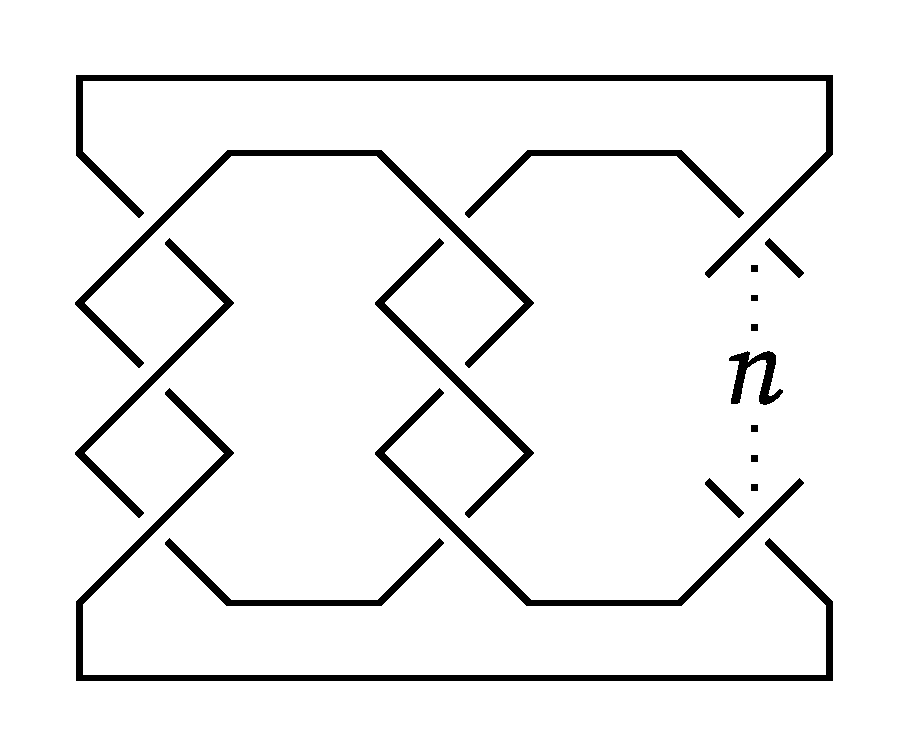
\includegraphics[width=0.4\textwidth]{images/pretzel-knot.pdf}
    \caption{The pretzel knot $P(3, -3, n)$. On the right, there are $n$ left half-twists if $n$ is positive, and $|n|$ \emph{right} half-twists if $n$ is negative.}
    \label{fig:pretzel-knot}
\end{figure}

We break the proof of this theorem into the following two lemmas.
\begin{lemma}\label{lem:tb}
    \[
        \maxtb P_n = \min \{ -n-4, -1\}.
    \]
\end{lemma}

\begin{lemma}\label{lem:cobordism}
    For each $P_n$, there exists a Legendrian representative $K_n$ of $P_n$ and a stabilized Legendrian unknot $U_n$ such that 
    \[
        \tb K_n = \tb U_n = \min \{-n-4, -1\},
    \]
    and there exists a decomposable Lagrangian concordance from $U_n$ to $K_n$.
\end{lemma}

The proof of Theorem~\ref{thm:mine} follows trivially from Lemmas~\ref{lem:tb}~and~\ref{lem:cobordism}, which we prove here.

\begin{proof}[Proof of Lemma~\ref{lem:tb}]

    We first compute the degree of $a$ in the Kauffman polynomial of $P_n$; as this allows us to obtain a bound on $\maxtb P_n$ by Theorem~\ref{kauffman-bound}. We use the method from \cite{lu-zhong} for computing the Kauffman polynomial of a pretzel knot, and find that $- \deg_a Y(P_n)$ is given by $\min\{-n-4, -1\}$. We implemented this computation in Mathematica; for details see Appendix~\ref{ch:appendix}.
    
    By Theorem~\ref{thm:ng} (Ng), the Kauffman bound is sharp for the pretzel link $P(3, -3, n)$ except when $n = 0$ or $n = \pm 2$. That is, ${\maxtb P_n = \min\{-n-4, -1\}}$ for $n \neq 0$ and $n \neq \pm 2$. We will deal with these cases presently.

    In the case where $n = 0$, ${P_0 = 3_1 \# m(3_1)}$. The Thurston-Bennequin number of a connected sum is well known \cite{torisu}, \cite{honda}. In particular,
    \[
        \maxtb{K_1 \# K_2} = \maxtb K_1 + \maxtb K_2 + 1.
    \]
    Thus $\maxtb P_0 = -6 + 1 + 1 = -4$ as desired \cite{atlas}.

    In the case where $n = \pm 2$, we have $P_2 = 8_{20}$ and $P_{-2} = m(8_{20})$, and therefore ${\maxtb P_2 = -6 = -2-4}$ and ${\maxtb P_{-2} = -2 = 2-4}$ as desired \cite{atlas}.

\end{proof}


\begin{proof}[Proof of Lemma~\ref{lem:cobordism}]

    \begin{figure}[ht]
        \centering
        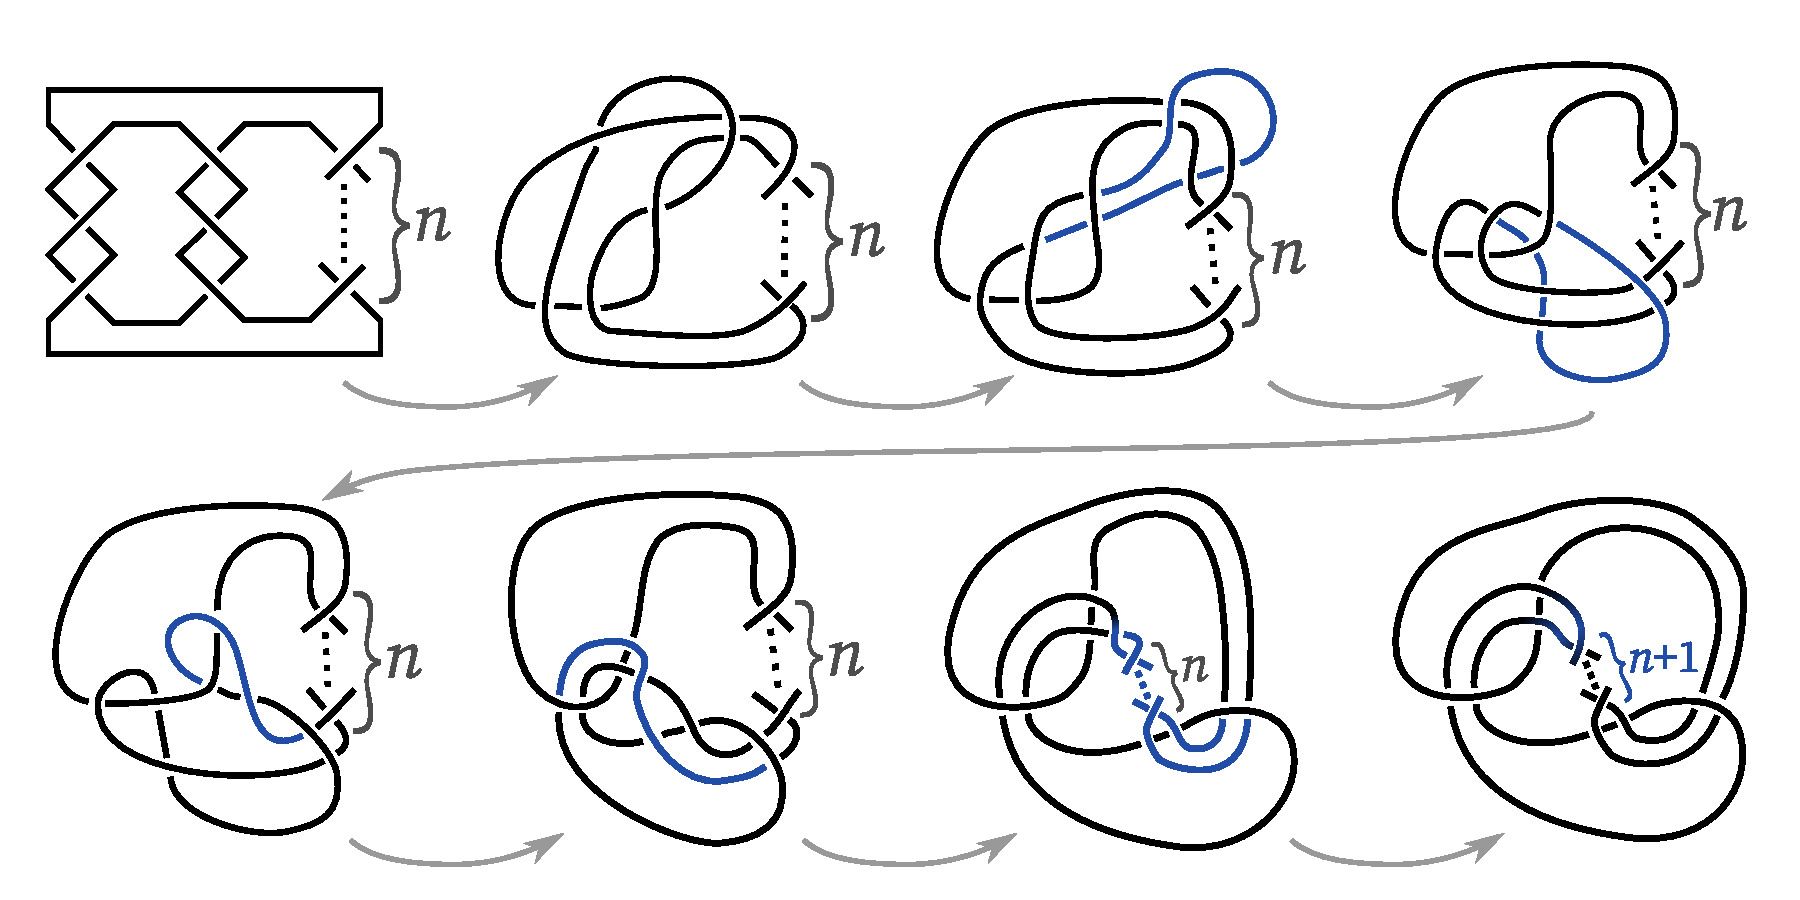
\includegraphics[width=0.9\textwidth]{images/isotopy-presentable.pdf}
        \caption{Smooth isotopy from the pretzel diagram for $P(3, -3, n)$ to a twisted ribbon.}
        \label{fig:isotopy}
    \end{figure}

    Depending on the value of $n$, there are three cases.

    In each, we first construct a suitable unknot $U_n$ with the desired $\tb$, using stabilizations or RI moves to add a total of $n-1$ half-twists, and we show the form of the desired Legendrian representative $K_n$. Figure~\ref{fig:isotopy} verifies that $K_n$ is in fact smoothly isotopic to $P(3, -3, n)$.

    We then use the decomposable moves to describe a decomposable Lagrangian cobordism from $U_n$ to $K_n$. A more detailed example of this construction is seen in Figure~\ref{fig:cobordism-construction}.

\begin{itemize}

    \item[$n \geq -1$ :]

        The desired $\tb$ is $-n-4$.
        We start with an unknot stabilized $n+1$ times in order to add $n+1$ left half-twists, as seen on the left in Figure~\ref{fig:pretzel-geq}.
        We add a 0-handle, and then use the Legendrian RII and RIII moves to thread the twisted band through both loops, before connecting them with a 1-handle.


        As this cobordism is in fact a concordance, we have $\tb U_n = \tb K_n$, so it suffices to check that $\tb U_n = -n-4$. The diagram for $U_n$ has three right cusps and $n+1$ crossings, each of which is negative. Thus $\tb U_n = -(n+1) - 3 = -n-4$ as desired.

        Note that in the case $n = -1$, the band is untwisted, as in Figure~\ref{fig:cobordism-construction}.
        \begin{figure}[ht!]
            \centering
            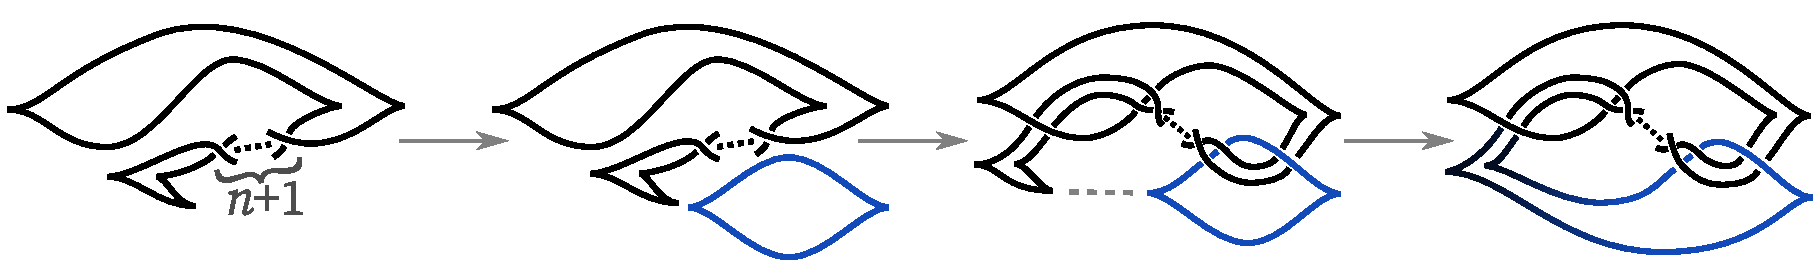
\includegraphics[width=0.95\textwidth]{images/cobordism-movie-g0-short.pdf}
            \caption{Cobordism movie for constructing $K_n$, where $n \geq 0$.}
            \label{fig:pretzel-geq}
        \end{figure}

    \item[$n = -2$ :]

        Recall that $P_{-2} = m(8_{20})$, and its maximal $\tb$ is $-2$. In the twisted band we will have $1$ \emph{right} twist.

        The diagram for the unknot $U_{-2}$, on the left, has 3 right cusps and a single crossing with positive sign. Thus $\tb U_{-2} = 1 - 3 = -2$.

        \begin{figure}[ht!]
            \centering
            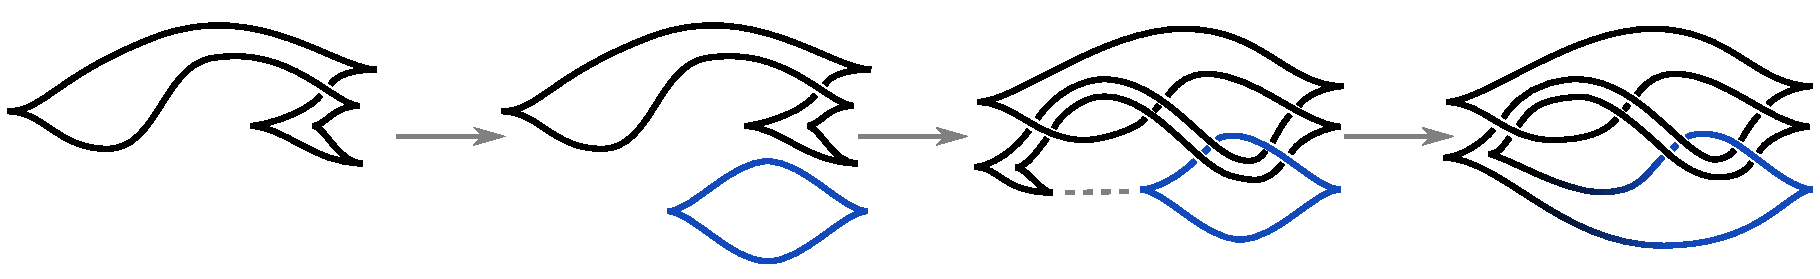
\includegraphics[width=0.95\textwidth]{images/cobordism-movie--2-short.pdf}
            \caption{Construction of $K_{-2}$.}
            \label{fig:pretzel--2}
        \end{figure}

    \item[$n \leq -3$ :]

        The desired $\tb$ is $-1$. Using the RI move we can add as many right half-twists as we like (i.e., $|n| - 1$) to our $U_n$ before we make the pinch move.

        Note that in Figure~\ref{fig:pretzel-leq} below, there are a total of $|n| - 1$ right half-twists, but one of them "stays behind" when we pass the ribbon tip through the loops.

        The diagram for $U_n$ has $|n|$ right cusps and $|n| - 1$ positive crossings, so $\tb U_n = (|n| - 1) - |n| = -1$ as desired.

        \begin{figure}[ht!]
            \centering
            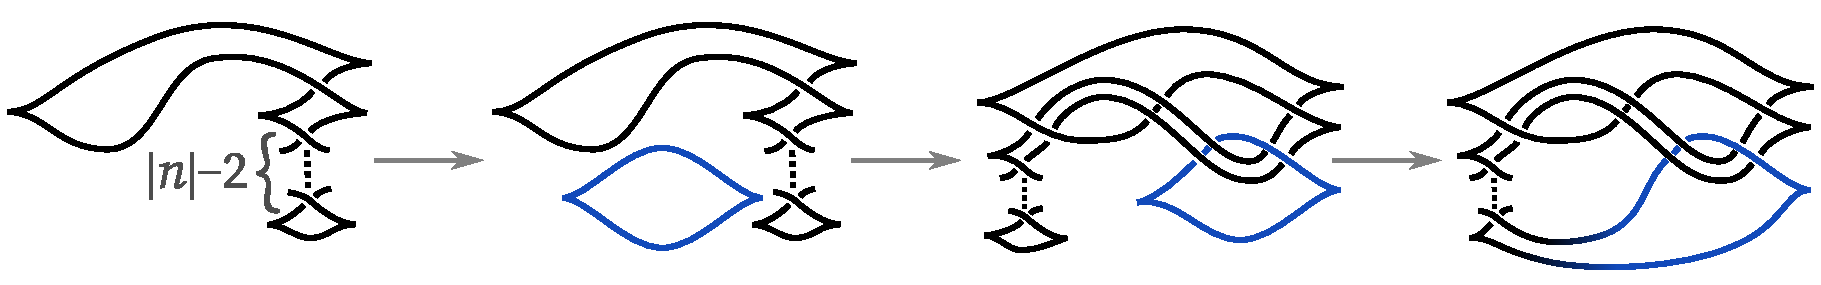
\includegraphics[width=0.95\textwidth]{images/cobordism-movie-l-3-short.pdf}
            \caption{Construction of $K_n$, where $n \leq -3$.}
            \label{fig:pretzel-leq}
        \end{figure}

\end{itemize}

\end{proof}

For a few specific $n$, Theorem~\ref{thm:mine} is sufficient to show that all Legendrian representatives of $P_n$ admit Lagrangian cobordisms from the unknot.
\begin{corollary}
    All Legendrian representatives of $P_1$, $P_3$, $P_{-3}$, and all but (possibly) one of $P_{-1}$ admit decomposable Lagrangian concordances from stabilized Legendrian unknots.
\end{corollary}
\begin{proof}

    Recall that if there exists a Lagrangian cobordism from $K_-$ to $K_+$, then there exists a Lagrangian cobordism from $S_-(K_-)$ to $S_-(K_+)$ and from $S_+(K_-)$ to $S_+(K_+)$, where $S_-$ and $S_+$ denote positive and negative stabilization respectively. Thus it suffices to check that all Legendrian representatives of $P_n$ are either $K_n$ or obtained from $K_n$ by repeated stabilization.

    For $P_{1}$ and $P_{\pm 3}$, all stabilized Legendrian representatives are known to be stabilizations of a single representative with maximal $\tb$ \cite{atlas}. This representative is necessarily $K_n$.

    In the case of $P_{-1}$, all stabilized representatives are stabilizations of \emph{either of two} maximal-$\tb$ representatives. That is, from \emph{either} maximal representative, all non-maximal representatives may be obtained by stabilization. Thus one of these representatives is $K_{-1}$, but it is unclear whether the other admits a Lagrangian concordance from the unknot.

\end{proof}


\chapter{Future Work}\label{ch:future}

The question of interest is whether there exist Lagrangian cobordisms from the unknot to all Legendrian ribbon knots. It suffices in this case to show that this is true for all nonstabilized representatives. The representatives with maximal $\tb$ are a subset of the nonstabilized representatives.
In this paper we showed that there exists Lagrangian cobordisms from the unknot to \emph{at least one} representative with maximal $\tb$ for a large family of ribbon pretzel knots, but our solution does not give information about the answer to this question in general. 

Our solution made use of a parameterization of ribbon pretzel knots, and we computed the maximal $\tb$ using an explicit formula for the Kauffman bound. There is another class of ribbon knots for which this approach might work --- 2-bridge knots.
The Kauffman bound is known to be sharp for these knots \cite{ng}, and an algorithm exists for computing it \cite{luzhong-2bridge}, much like the algorithm we used for pretzel knots.
Moreover, many of the prime knots for which we have failed to explicitly find maximal-$\tb$ cobordisms from the unknot are 2-bridge: for example, $8_8$ and $8_9$. In fact, there are several known families of 2-bridge ribbon knots, and it is conjectured that these families include all 2-bridge ribbon knots \cite{lamm}.

Yet in the case of the pretzel knots $P(3, -3, n)$, our proof relied on an explicit stabilized unknot for each $n$ such that each cobordism could be constructed using the exact same sequence of moves.
If a similar method could be used to prove the existence of such cobordisms for 2-bridge knots, the first step would be to find a single explicit example --- which so far we have failed to do.

However, finding a positive answer in general is much more difficult due to the wide variety of ways that the equivalence classes of Legendrian knots can be organized. For example, there exist knots having \emph{nonstabilized} representatives with the same $\tb$ and rotation number as stabilized representatives \cite{mountain}. There exist knots with infinitely many pairs of distinct Legendrian representatives $(K, K')$ such that $\tb K = \tb K'$ and $\rot K = \rot K'$ (in particular, this is true of $P_-4$). More examples of the strangeness of Legendrian equivalence classes may be readily found in \cite{atlas}. Yet the takeaway is that the nonstabilized Legendrian representatives of a topological knot type can have little in common, making it difficult to to prove anything about them.




\begin{appendices}

    \chapter{Mathematica Code for Kauffman Bound Computation}\label{ch:appendix}

\lstset{language=Mathematica,style=better}

Throughout, the pretzel knot $P(a, b, c)$ is encoded by the list \lstinline|{a, b, c}|.

We obtain Lu and Zhong's version of the Dubrovnik Polynomial using their algorithm (\cite{lu-zhong}).
After marking some shorthand and writing out the base change matrix $M$, we directly implement Lu and Zhong's formula for the Dubrovnik polynomial in the function \lstinline|LuZhong[q]|.

\begin{lstlisting}
ai := 1/a;
si := 1/s;
d  := (a - ai)/(s - si) + 1;
di := 1/d;
M   = {
    {   (si - di*si - di*ai) / (s + si),
        (-si - di*s + di*ai) / (s + si),
        di},
    {   (-s - di*si - di*ai) / (s + si),
        (s - di*s + di*ai)   / (s + si),
        di},
    {   (si*d + a - di*si - di*ai) / (s + si),
        (s*d - a - di*s + di*ai)   / (s + si),
        di}
    };

LuZhong[q_] :=
    d * M[[3]] . Table[
        Times @@ (M[[j]] . {s, -si, ai}^#1 &) /@ q, {j, 3}
    ]
\end{lstlisting}

Now we compute the ``standard'' Dubrovnik polynomial, as Lu and Zhong's version has $s - s^{-1}$ instead of $z$ throughout. To do this we need to rewrite the equation in the variables $a, z$ where $z = s - s^{-1}$. This doesn't affect the degree of $a$, but it makes it easier to check that the coefficients of the relevant powers of $a$ are not identically zero.

\begin{lstlisting}
Dubrovnik[q_] :=
 	LuZhong[q] /. Solve[z == s - si, s][[1]] // Simplify
\end{lstlisting}

Now we will normalize the Dubrovnik polynomial to get the Kauffman $Y$ polynomial. But first, we need the writhe. For the family we are interested in, the writhe is easy to compute.

\begin{lstlisting}
Writhe[{3, -3, n_}] := -n
Kauffman[q_] :=
    Simplify[Dubrovnik[q] * ai^Writhe[q]]
\end{lstlisting}

As we know, we can use the Kauffman polynomial to get an upper bound on the maximal Thurston-Bennequin number. Using Tabachnikov's version of the bound (\cite{tabachnikov}), we can write

\begin{lstlisting}
TBBound[q_] :=
    (-Exponent[Kauffman[q], a, Max]) // Simplify
\end{lstlisting}

Finally, we can allow Mathematica to crunch the terms:

\begin{lstlisting}[escapeinside={(*}{*)}]
$Assumptions = {n (*$\in$*) Integers};
TBBound[{3, -3, n}]
\end{lstlisting}

and the result is \lstinline|-Max[1, 4 + n]| which is of course $\min\{-1, -4-n\}$ as desired.

% Check the coefficients
Is there any $n$ such that coefficient of $a^{n+4}$ or of $a$ vanishes in the Kauffman polynomial of $P(3, -3, n)$?
It is simple to check that this is not the case, verifying the above expression for $\deg_a$.

\begin{lstlisting}
P = Kauffman[{3, -3, n}] // Expand // PowerExpand // Apart // Expand;
coeff1 = Coefficient[P, a, 1] // FullSimplify
coeffn4 = Coefficient[P, a, n+4] // FullSimplify;
Solve[coeff4n == 0, n]
\end{lstlisting}

On the one hand, \lstinline|coeff1 == 1/z|, which is certainly nonzero. Moreover, \lstinline|coeff4n == 0| when the following holds:
\setmuskip{\thinmuskip}{2mu minus 2mu}
\setmuskip{\medmuskip}{3mu plus 2mu minus 3mu}
\[
    n = \frac{ \ln\left((2 + 16 z^2 + 20 z^4 + 8 z^6 + z^8 + 4 z \sqrt{4 + z^2} + 10 z^3 \sqrt{4 + z^2} + 6 z^5 \sqrt{4 + z^2} + z^7 \sqrt{4 + z^2})/2\right)}{\ln 2 - \ln \left(z (-z + \sqrt{4 + z^2}) - 2\right)}
\]
\begin{figure}[h]
    \centering
    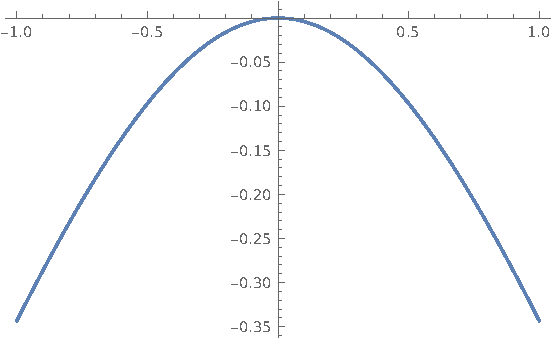
\includegraphics[width=0.3\textwidth]{images/mathematica-n.pdf}
    \caption{A plot of the real part of the above expression, showing that it is not satisfied by any integral constant $n$.}
\end{figure}




\end{appendices}

\printbibliography[heading=bibintoc]
\end{document}
